\documentclass[class=../../report, crop=false]{standalone}
\usepackage{graphicx}
\usepackage{caption}

\DeclareCaptionFormat{cont}{#1 (cont.)#2#3\par}
\begin{document}

\section{Functional Decomposition Diagram} \label{app:funcdecomp}

\begin{figure}[!htb]
	\centering
	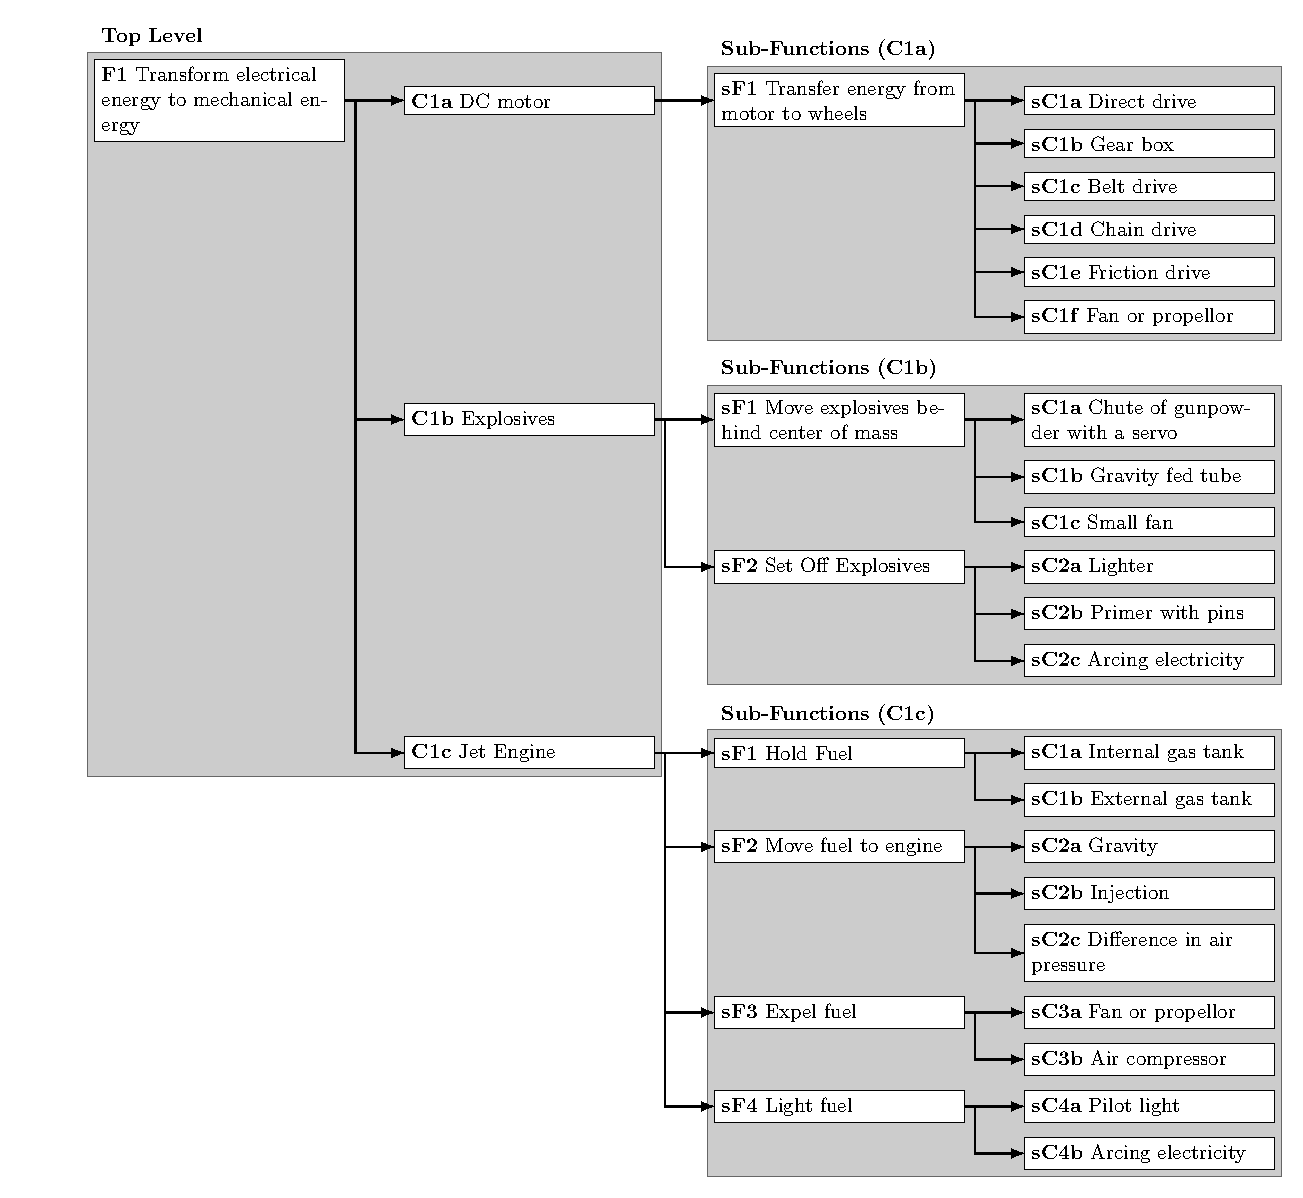
\includegraphics[width=\textwidth]{../../../bin/funcdecomp-1}
	\caption{Functional Decomposition Diagram Part 1}
\end{figure}
\begin{figure}[!htb]
	\ContinuedFloat
	\centering
	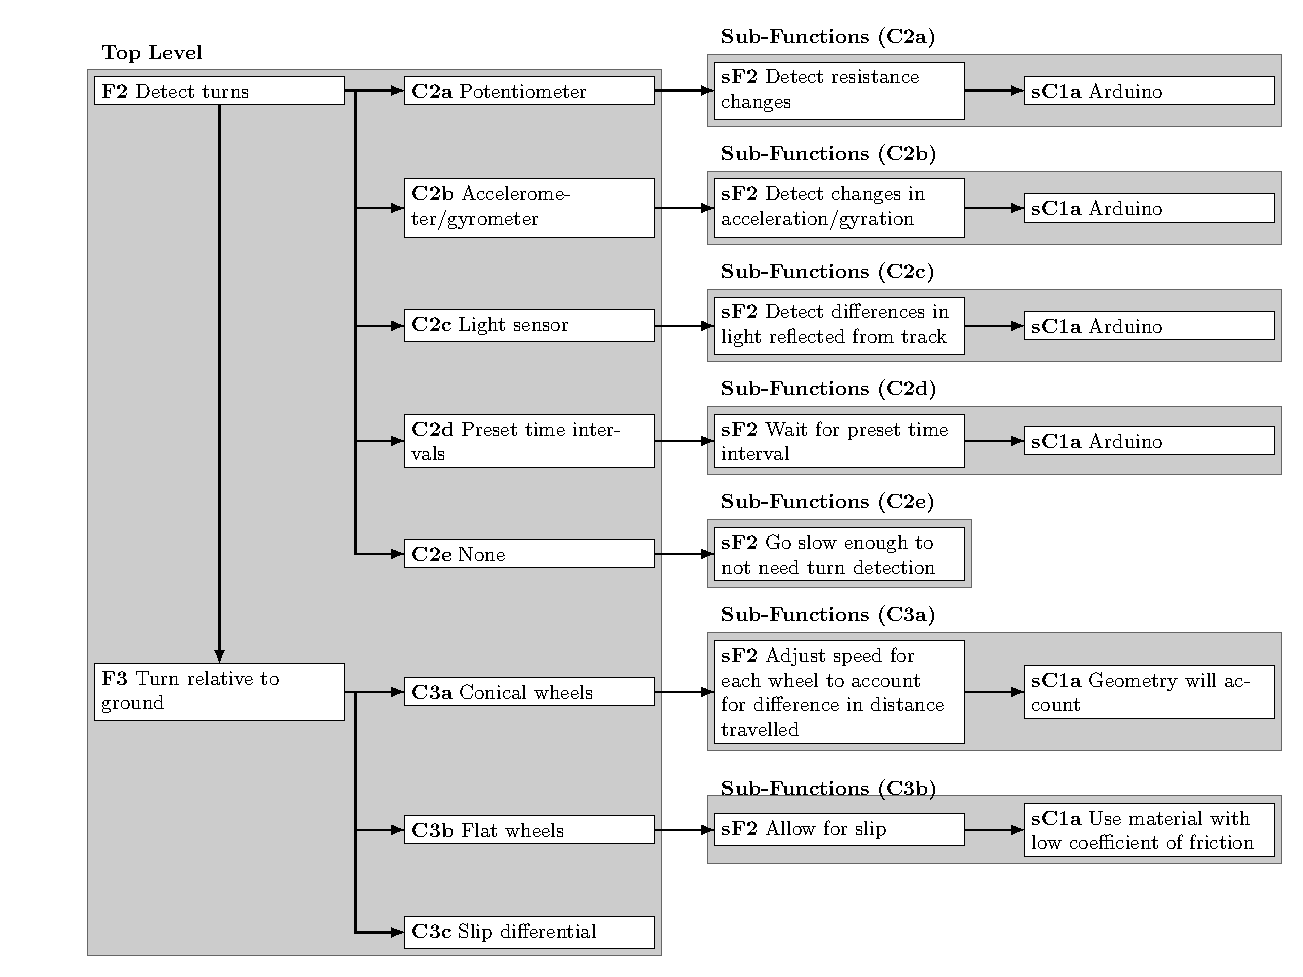
\includegraphics[width=\textwidth]{../../../bin/funcdecomp-2}
	\caption{Functional Decomposition Diagram Part 2}
\end{figure}
\begin{figure}[!htb]
	\ContinuedFloat
	\centering
	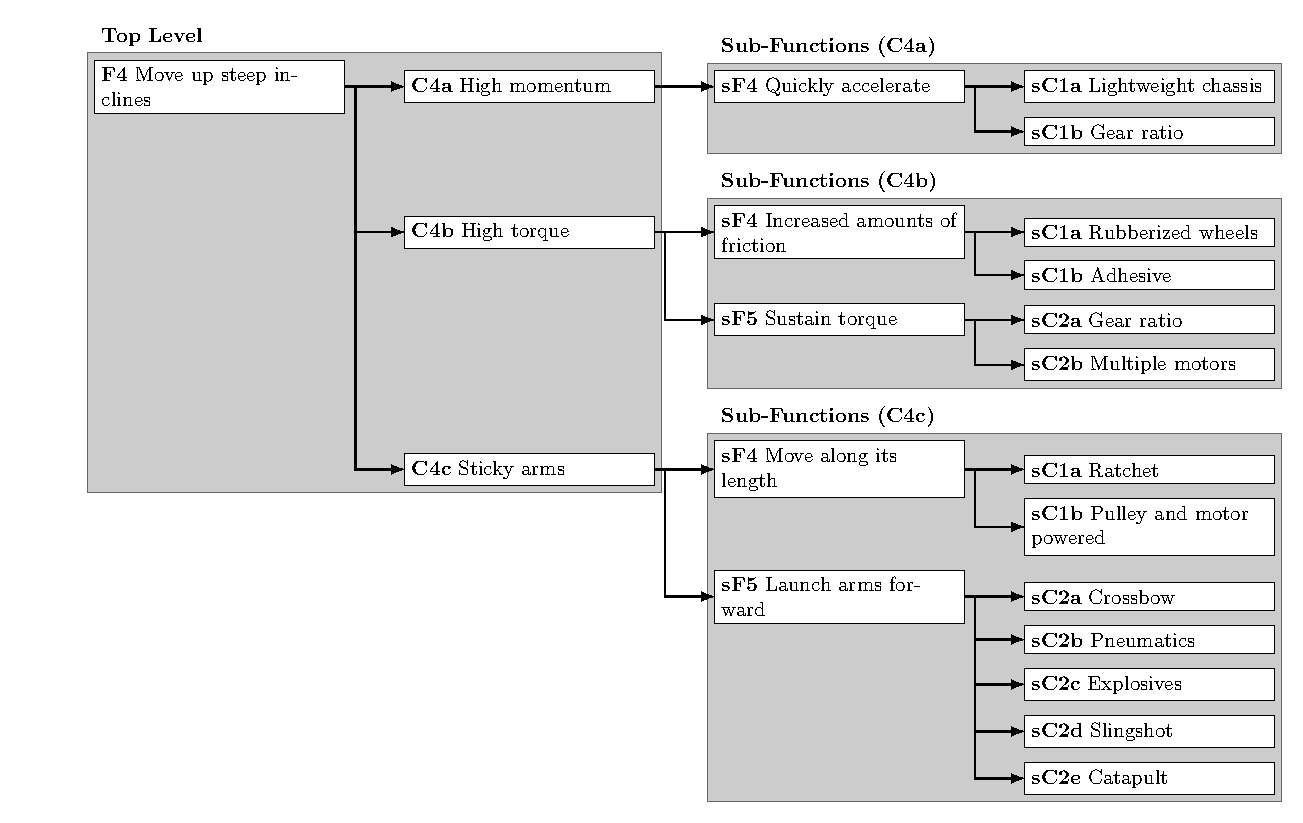
\includegraphics[width=\textwidth]{../../../bin/funcdecomp-3}
	\caption{Functional Decomposition Diagram Part 3}
\end{figure}
\begin{figure}[!htb]
	\ContinuedFloat
	\centering
	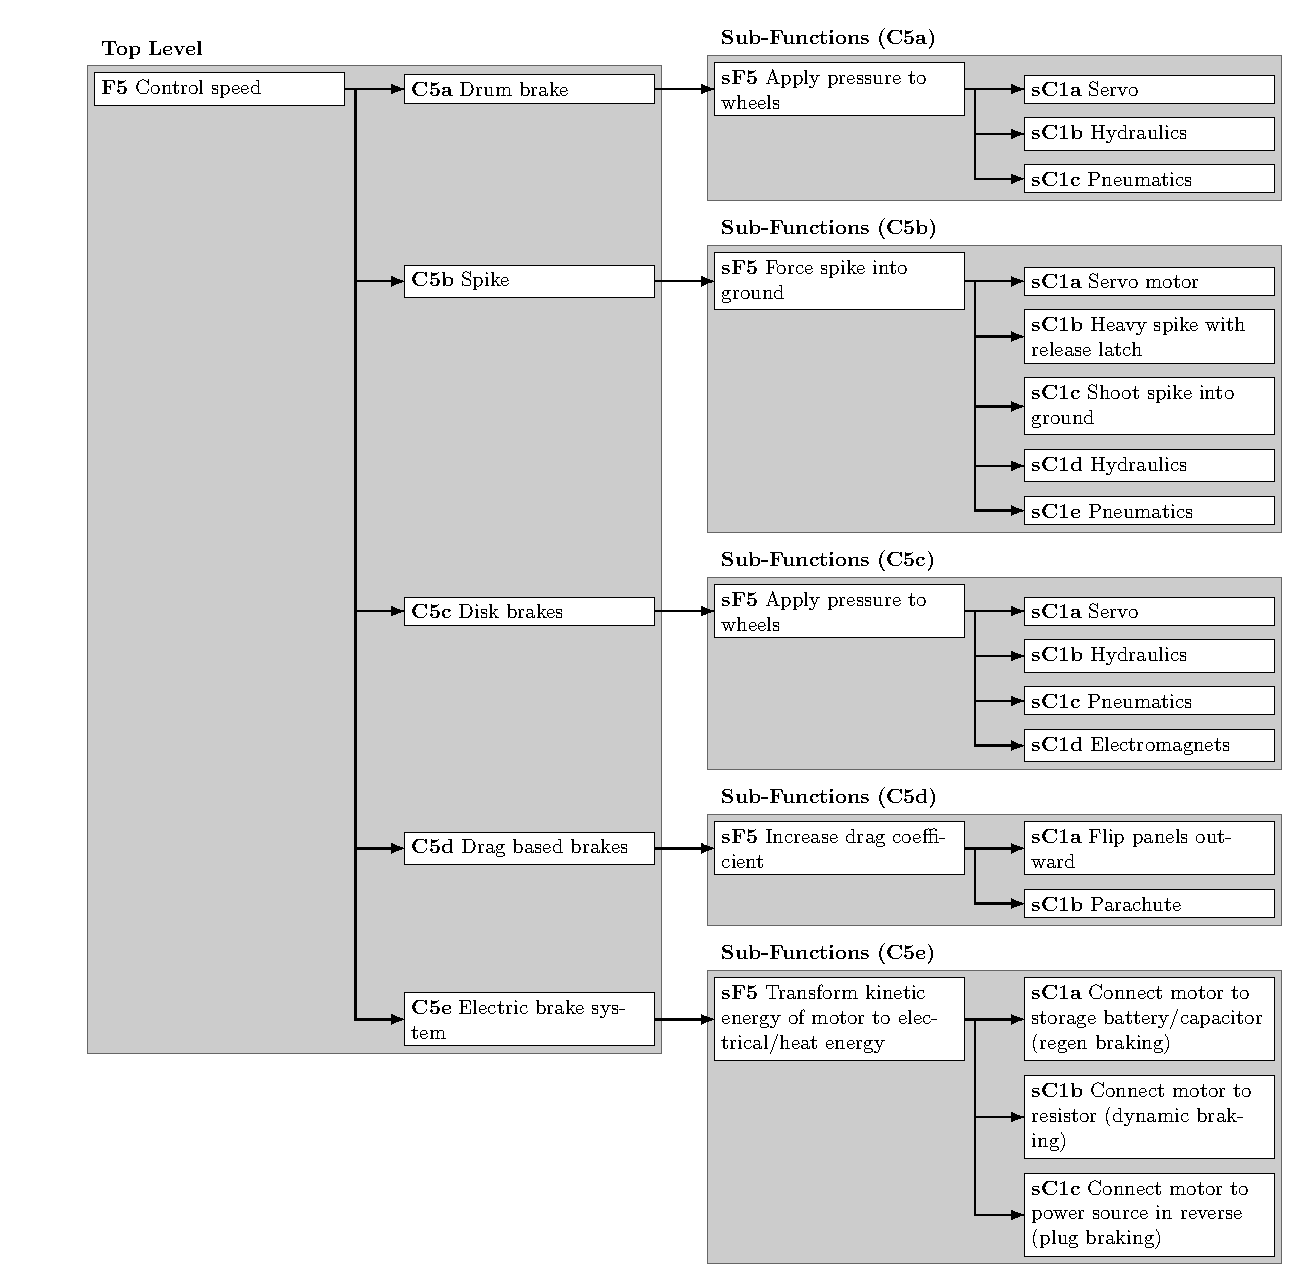
\includegraphics[width=\textwidth]{../../../bin/funcdecomp-4}
	\caption{Functional Decomposition Diagram Part 4}
\end{figure}
\begin{figure}[!htb]
	\ContinuedFloat
	\centering
	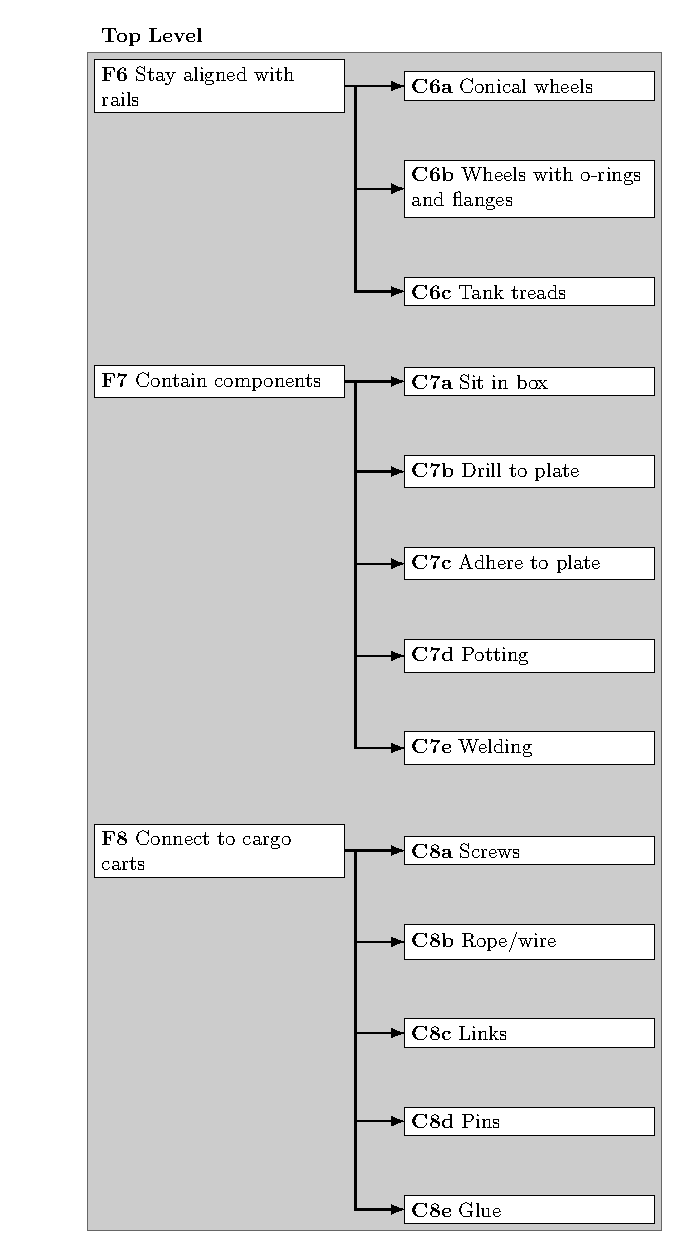
\includegraphics[trim=10.5cm 0 0 0,scale=0.75]{../../../bin/funcdecomp-5}
	\caption{Functional Decomposition Diagram Part 5}
\end{figure}
\end{document}
